%%%%%%%%%%%%%%%%%%%%%%%%%%%%%%%%%%%%%%%%%%%%%%%%%
%%%%%%%%%%%%%%%%%%%%%%%%%%%%%%%%%%%%%%%%%%%%%%%%%
%%
%%  Modèle pour le  Bulletin de l'Association
%%           mathématique du Québec
%%
%%                 Décembre 2017
%%       Adapté par Marc-André Désautels
%%
%%%%%%%%%%%%%%%%%%%%%%%%%%%%%%%%%%%%%%%%%%%%%%%%%
%%%%%%%%%%%%%%%%%%%%%%%%%%%%%%%%%%%%%%%%%%%%%%%%%


\documentclass[10pt]{article}

%=====================================Ensemble des packages================================

% Ce package sert à accueillir les accents et à faire
% les césures comme on aime qu'elles soient faites en français.
\usepackage[T1]{fontenc}

% Choix de la fonte
\usepackage{lmodern}

%% Permet de traiter les textes accentués
% Pour Windows
\usepackage[utf8]{inputenc}
% Pour Unix
%\usepackage[latin1]{inputenc}
% Pour Apple
%\usepackage[applemac]{inputenc}

% Ensuite, entrer le texte accentué comme à l'ordinaire.
\usepackage[english,french]{babel}

% Permet de rendre le fichier maître plus compatible,
% en particulier avec l'insertion de figures,
% (sauf celle de figures flottantes (package floatingfigure))
% et avec la définition des caractères à doubles jambes.
\usepackage{graphicx}

% Packages qui permettent l'utilisation des symboles et des commandes
% mathématiques de AMS-LaTeX,
\usepackage{amssymb,latexsym,amsmath}

% Package qui donne accès à une police calligraphique, comme eucal.
\usepackage{mathrsfs}

% Package qui permet de fusionner des lignes ou des colonnes de tableaux
\usepackage{multirow}

% Package qui donne accès à la fonte Euler.
\usepackage{euscript}

% Package qui permet de définir ses propres en-têtes et pieds de page.
\usepackage{fancyhdr}

% Package qui permet de passer du texte sur le fichier
% pdf à la ligne du fichier source correspondant.
\usepackage{pdfsync}

% Package permettant de définir son propre style
% de présentation des théorèmes.
\usepackage{theorem}

% Package qui permet au texte de s'enrouler autour de flotants.
\usepackage{wrapfig}
\usepackage{floatflt}

% Package qui "rectifie" les caractères qui dépassent dans la marge.
\usepackage[protrusion=true]{microtype}

% Permet de tracer des graphes flèchés.
% Voir http://www.tug.org/TUGboat/tb22-4/tb72perlax.pdf
\usepackage[all]{xy}

%  Permet de définir les dimensions de la partie imprimée de la page.
% Voir http://ctan.cms.math.ca/tex-archive/macros/latex/contrib/geometry/geometry.pdf
\usepackage{geometry}

% Permet, entre autres, de mettre du texte en filigrane.
% Voir http://math.et.info.free.fr/TikZ/bdd/TikZ-Impatient.pdf
% p. 165
\usepackage{tikz}

% Permet d'utiliser le gabarit de tableaux utilisant les commandes
% of \toprule, \midrule and \bottomrule pour les lignes horizontales dans les tableaux.
\usepackage{booktabs}

\usepackage{color}

% Permet la présentation d'adresses url sous leur forme habituelle.
% Voir http://www.tex.ac.uk/cgi-bin/texfaq2html?label=setURL
\usepackage{url}

% Permet de rendre actifs les liens créés avec le package précédent.
% Voir /usr/local/share/texmf-dist/doc/latex/hyperref/manual.pdf
\usepackage[colorlinks=true,urlcolor=blue, citecolor=cyan, linkcolor=magenta]{hyperref}

% Pour une adresse de courriel: \href{mailto:foo@bar.abc}{Good Link!}
% Pour de belles flèches sur les vecteurs, cadeau de Jean-Philippe Morin
\usepackage{esvect}

%==================================Fin de l'ensemble des packages============================


%=================Pour de belles flèches sur les vecteurs, cadeau de Jean-Philippe Morin=====
\renewcommand{\vec}[1]{\protect\vv{#1}}
% notation de vecteur (\vv définie par package esvect)
% Exemple: \vv{v} ou \vv{AB} ou \vv{A_1A_2}
%============================================================================================


%%%======= Début macro pour numérotation des équations selon les sections du texte==========
%\makeatletter
%\renewcommand\theequation{\thesection.\arabic{equation}}
%\@addtoreset{equation}{section}
%\makeatother
%%%======================  macro: mode d'emploi ============================================
%%% Pour activer cette macro commande, enlever le symbole % au début de la ligne suivante
%\numberwithin{equation}{section}
%%============================================================================================




%%===========Les énoncés ayant la même présentation que les théorèmes=========================
\newtheorem{theorem}{Théorème}
%[section]
\newtheorem{lemma}{Lemme}
%[section]
\newtheorem{proposition}{Proposition}
%[section]
\newtheorem{corollary}{Corollaire}
%[section]
\newtheorem{definition}{Définition}
%[section]
\newtheorem{nota}{Notation}
%[section]
\newtheorem{ex}{Exemple}
%[section]
\newtheorem{nb}{N.B.}
%[section]
\newtheorem{remark}{Remarque}
%%============================================================================================


%%==========================Les démonstrations============================
\newenvironment{proof}
{\par\noindent
\textit{Démonstration}\ }
{
\hfill{$\Box$}
}

%%==============================Les siècles====================================================
%%        Pour la notation des siècles en chiffres romains
%%        La commande est  \siecle{#}
%%        Exemple  \siecle{21}.
%%==========================================================================================
\newcommand{\siecle}[1]{%
\ifnum #1=1%
\uppercase\expandafter{\romannumeral #1}\textsuperscript{er}%
\else%
\uppercase\expandafter{\romannumeral #1}\up{e}%
\fi}

%%=====================================================================
%   Définition des marges pour le Bulletin (NE PAS MODIFIER)
\geometry{height=18.6cm,width=14.4cm}
\geometry{hmargin={3.6cm,3.6cm}}
\geometry{vmargin={4.3cm,5cm}}
%%Ces trois lignes doivent rester avant le \begin{document}.
\parindent=0.0in
\parskip=0.1in
\setcounter{page}{1}
%%=====================================================================

%%========================Caractères particuliers usuels======================
%%
%%==============================Double jambe.============================
\DeclareSymbolFont{AMSb}{U}{msb}{m}{n}
\DeclareSymbolFontAlphabet{\Bbb}{AMSb}
\newcommand{\ds}{\displaystyle}

\usepackage[]{lineno}

\newcommand*\patchAmsMathEnvironmentForLineno[1]{%
  \expandafter\let\csname old#1\expandafter\endcsname\csname #1\endcsname
  \expandafter\let\csname oldend#1\expandafter\endcsname\csname end#1\endcsname
  \renewenvironment{#1}%
     {\linenomath\csname old#1\endcsname}%
     {\csname oldend#1\endcsname\endlinenomath}}%
\newcommand*\patchBothAmsMathEnvironmentsForLineno[1]{%
  \patchAmsMathEnvironmentForLineno{#1}%
  \patchAmsMathEnvironmentForLineno{#1*}}%
\AtBeginDocument{%
\patchBothAmsMathEnvironmentsForLineno{equation}%
\patchBothAmsMathEnvironmentsForLineno{align}%
\patchBothAmsMathEnvironmentsForLineno{flalign}%
\patchBothAmsMathEnvironmentsForLineno{alignat}%
\patchBothAmsMathEnvironmentsForLineno{gather}%
\patchBothAmsMathEnvironmentsForLineno{multline}%
}

%%==========================Packages propres à l'auteur==============================
%%
%% Vous pouvez ajouter ici tous les packages que vous avez besoin.
%% Par exemple

% \usepackage{pstricks}
% \usepackage{enumitem}

%\usepackage{pstricks}
%\usepackage{pst-all}
\usepackage{csquotes}
\usepackage{cancel}
\allowdisplaybreaks

%%
%%==========================Fin des packages propres à l'auteur=======================

%%==========================Commandes propres à l'auteur==============================
%%
%% Vous pouvez ajouter ici toutes les commandes que vous avez définies.
%% Par exemple

% \newcommand{\lr}[1]{\left(#1\right)}
% \newcommand{\abs}[1]{\left\vert#1\right\vert}

\DeclareMathOperator{\Arcsin}{Arcsin}
\DeclareMathOperator{\Arccos}{Arccos}
\DeclareMathOperator{\Arcsec}{Arcsec}
\DeclareMathOperator{\Arccsc}{Arccsc}
\DeclareMathOperator{\Arccot}{Arccot}
\DeclareMathOperator{\Arctan}{Arctan}
\DeclareMathOperator{\Arctanh}{Arctanh}
\DeclareMathOperator{\sech}{sech}
\DeclareMathOperator{\esp}{\mathbb{E}}
\DeclareMathOperator{\var}{Var}
\DeclareMathOperator{\cov}{Cov}
\DeclareMathOperator{\unif}{U}
\newcommand{\lr}[1]{\left(#1\right)}
\newcommand{\abs}[1]{\left\vert#1\right\vert}
\newcommand{\norm}[1]{\left\Vert#1\right\Vert}
\newcommand{\set}[1]{\left\{#1\right\}}
\newcommand{\crochet}[1]{\left[#1\right]}
\newcommand{\comeq}[1]{\quad\lr{\text{#1}}}


%%
%%==========================Fin des commandes propres à l'auteur========================

\usepackage{url}
\usepackage{hyperref}

%%============================pour des barres de fraction obliques=======================
%running fraction with slash - requires math mode.
\newcommand*\rfrac[2]{{}^{#1}\!/_{#2}}
%	Exemple :	\rfrac{3}{7}
%%===============================================================================


%%=== Pour des barres de fraction latérales, une petite, une grande et une très grande ===
\newcommand{\fracinline}[2]{\raisebox{0.4ex}{$#1$} / \raisebox{-0.7ex}{$#2$}}
\newcommand{\bigfracinline}[2]{\raisebox{0.8ex}{$#1$}  \Big/ \raisebox{-1.4ex}{$#2$}}
\newcommand{\biggfracinline}[2]{\raisebox{0.8ex}{$#1$}  \Bigg/ \raisebox{-1.4ex}{$#2$}}

%%	Exemple:	\fracinline{1 + \cos x}{\sin x}
%%	Exemple:	\bigfracinline{1 + \cos x}{\sin x}
%%	Exemple:	\biggfracinline{1 + \cos x}{\sin x}
%%=======================================================================================

\everymath{\displaystyle}


\begin{document}

%%==========================Éléments propres à l'auteur==============================
%%
%%
%%==========================Fin des éléments propres à l'auteur======================


%%=====================Pour mettre le titre des tableaux en français==================
%%
\renewcommand{\tablename}{\textsc{Tableau}}
%%
%%=========================Fin de la nouvelle définition==============================

\begin{center}
\textsf{\LARGE \textbf{Le problème du char d'assaut allemand}}
\end{center}

\begin{flushright}
\textsc{Marc-André Désautels, département de mathématiques} \\
\textsc{Cégep de Saint-Jean-sur-Richelieu} \\
\href{mailto:marc-andre.desautels@cstjean.qc.ca}{marc-andre.desautels@cstjean.qc.ca} \\
\href{https://www.cstjean.qc.ca/}{https://www.cstjean.qc.ca/}
\end{flushright}


\baselineskip=1.2\baselineskip

%%=====================================================================
%%          Résumé
%%=====================================================================

\begin{abstract}

Durant la seconde guerre mondiale, les alliés avaient un besoin criant
d'estimer avec précision la quantité de matériel militaire que
l'Allemagne nazie produisait. Les estimations provenant des services de
renseignements habituels étaient contradictoires et incertaines. Les
gouvernements Britanniques et Américains se tournèrent donc vers des
statisticiens pour savoir si leurs estimations pouvaient être
améliorées. Nous présenterons une introduction aux notions mathématiques
utilisées.

\end{abstract}
%%=====================================================================
%%          Fin du résumé
%%=====================================================================

\textbf{Mots clés: } Statistiques, Estimation, Simulation

\bigskip

\hypertarget{introduction}{%
\section{\texorpdfstring{Introduction
\label{intro}}{Introduction }}\label{introduction}}

Au début de l'année 1943, la \emph{Economic Warfare Division} de
l'ambassade américaine à Londres commença à analyser divers marquages
obtenus à partir d'équipements allemands capturés ou détruits sur le
front. Plus particulièrement, les numéros de séries ont été utilisés
pour estimer la force de production de la machine de guerre allemande.
L'article \emph{An Empirical Approach to Economic Intelligence in World
War II} \cite{Ruggles1947} explique en grand détail le développement des
techniques utilisés pour faire cette estimation, les problèmes
rencontrés et les solutions qui y ont remédiés. Nous invitons le lecteur
intéressé par l'aspect pratico-pratique de ces techniques à lire cet
article.

Le problème du char d'assaut allemand est nommé d'après son application
par les alliés à l'estimation du nombre de chars d'assaut produits par
l'Allemagne. Mais en fait, ce problème regroupe l'estimation du nombre
de nombreux produits de guerre allemands, par exemple les camions, les
fusils, les bombes et les fusées.

Dans cet article, nous nous intéresserons à l'estimation du nombre
d'items \(N\) à partir d'un échantillon aléatoire dans le cas où les
items sont numérotés de façon séquentielle.

\hypertarget{les-mathematiques}{%
\section{\texorpdfstring{Les mathématiques
\label{maths}}{Les mathématiques }}\label{les-mathematiques}}

\hypertarget{prealables}{%
\subsection{Préalables}\label{prealables}}

Supposons que nous avons une population d'objets numérotés de la façon
suivante : \(1\), \(2\), \(3\), \ldots{} , \(N\), où \(N\) est
\textbf{inconnu}. Nous pigeons, \textbf{\textbf{sans remise}}, un
échantillon \(X_1\), \(X_2\), \(X_3\), \ldots{}, \(X_n\), de taille
\(n\) à partir de la population. Nous voulons estimer la valeur de \(N\)
à partir de l'échantillon prélevé.

Pour calculer les diverses mesures statistiques dont nous aurons besoin,
nous allons classer les unités statistiques de notre échantillon en
ordre croissant. Nous avons:

\[X_{(1)} <  X_{(2)} < X_{(3)} < \ldots < X_{(n-1)} < X_{(n)}\]

où les valeurs \(X_{(1)}\), \(X_{(2)}\), \(X_{(3)}\), \ldots{},
\(X_{(n)}\) sont les valeurs ordonnées de l'échantillon \(X_1\),
\(X_2\), \(X_3\), \ldots{}, \(X_n\). En particulier, \(X_{(1)}\) est la
plus petite valeur de l'échantillon et \(X_{(n)}\) est la plus grande.

À partir de nos définitions précédentes, il est possible de calculer
l'espérance de la valeur \(X_{(A)}\) (\(E(X_{(A)})\)), la variance de la
valeur \(X_{(A)}\) (\(Var(X_{(A)})\)) et enfin la covariance des valeurs
\(X_{(A)}\) et \(X_{(B)}\) (\(Cov(X_{(A)},X_{(B)})\)). Nous utiliserons
ces mesures statistiques pour calculer l'espérance et la variance des
estimateurs que nous construirons. Malheureusement, retrouver ces
mesures statistiques nécessite des identités combinatoires et de
fastidieux calculs. Pour ne pas alourdir le texte, nous donnerons ces
mesures sans démonstration. Par contre, pour la lectrice ou le lecteur
intéressé, vous pourrez trouver à l'annexe \ref{calculs_proba} une idée
de la technique utilisée ainsi que la démonstration de \(E(X_{(A)})\).

Nous avons donc les trois mesures à la table \ref{tab:mesures_stat}.

\begin{table}[ht]
\begin{center}
\begin{tabular}{|r|c|}
\hline
Mesure & Formule \\
\hline
\hline
$E(X_{(A)})$ & $\dfrac{A(N+1)}{n+1}$ \\ \hline
$Var(X_{(A)})$ & $\dfrac{A(n+1-A)(N+1)(N-n)}{(n+1)^2(n+2)}$ \\ \hline
$Cov(X_{(A)},X_{(B)})$ & $\dfrac{A(n+1-B)(N+1)(N-n)}{(n+1)^2(n+2)}$ \\ \hline
\end{tabular}
\end{center}
\caption{\label{tab:mesures_stat} {Les mesures de l'espérance, de la variance et de la covariance.} }
\end{table}

À l'aide des trois mesures de la table \ref{tab:mesures_stat}, nous
allons maintenant trouverquatre estimés de \(N\) en utilisant simplement
notre ``gros bon sens''. La structure des prochaines sections est
calquée sur \cite{Johnson}.

\hypertarget{les-trois-situations-possibles}{%
\subsection{Les trois situations
possibles}\label{les-trois-situations-possibles}}

Supposons que nous avons une population d'objets numérotés de la façon
suivante : \(s+1\), \(s+2\), \(s+3\), \ldots{} , \(s+N\). Trois
situations distinctes peuvent se produire:

\begin{enumerate}
\def\labelenumi{\arabic{enumi}.}
\item
  \(s\) est \textbf{connu} et égal à \(0\) et \(N\) est
  \textbf{inconnu}.
\item
  \(s\) est \textbf{connu} mais différent de \(0\) et \(N\) est
  \textbf{inconnu}.
\item
  \(s\) est \textbf{inconnu} et \(N\) est \textbf{inconnu}.
\end{enumerate}

Nous étudierons, dans l'ordre, les trois situations précédentes.

\hypertarget{la-situation-ou-s-est-connu-et-egal-a-0-et-n-est-inconnu}{%
\subsection{\texorpdfstring{La situation où \(s\) est \textbf{connu} et
égal à \(0\) et \(N\) est
\textbf{inconnu}}{La situation où s est connu et égal à 0 et N est inconnu}}\label{la-situation-ou-s-est-connu-et-egal-a-0-et-n-est-inconnu}}

Puisque \(s\) est connu et égal à \(0\), nous nous trouvons dans la
situations où notre liste est numérotée de la façon suivante : \(1\),
\(2\), \ldots{}, \(N\).

\hypertarget{le-milieu-de-la-liste}{%
\subsubsection{Le milieu de la liste}\label{le-milieu-de-la-liste}}

Supposons que nous connaissons la valeur milieu \(m\) de la liste \(1\),
\(2\), \ldots{}, \(N\). Nous nous retrouvons dans la situation
ci-dessous:

\[\underbrace{1,2,3,\ldots,m-1}_{m-1 \text{ éléments}},m,\underbrace{m+1,\ldots,N-2,N-1,N}_{m-1 \text{ éléments}}\]

Il y aura donc \(m-1\) valeurs en-dessous de \(m\) et \(m-1\) valeurs
au-dessus de \(m\). Donc, si nous incluons la valeur milieu \(m\), nous
avons:

\[N=(m-1)+1+(m-1)=2m-1\]

Puisque nous ne connaissons pas \(m\), il est raisonnable de le
remplacer par une estimation, par exemple la médiane \(\widetilde{X}\)
ou la moyenne \(\overline{X}\). Nous pouvons maintenant obtenir nos deux
premiers estimateurs.

TODO: EST-CE QUE JE CALCULE LES VARIANCES AUSSI????????

\hypertarget{la-mediane}{%
\subsubsection{La médiane}\label{la-mediane}}

Notre premier estimateur est \(\widehat{N_1}=2\widetilde{X}-1\), où
\(\widetilde{X}\) représente la médiane de notre échantillon. Rappelons
que pour \(k\) données discrètes, la médiane se calcule de deux façons
différentes, dépendamment du fait que le nombre de données soit pair ou
impair. \begin{align}
\widetilde{X} &= 
\begin{cases}
\dfrac{X_{\left(\tfrac{k}{2}\right)}+X_{\left(\tfrac{k}{2}+1\right)}}{2} & \text{ si $k$ est pair} \\
X_{\left(\tfrac{k+1}{2}\right)} & \text{ si $k$ est impair}
\end{cases}
\label{eq:mediane}
\end{align}

En utlisant les mesures du tableau \ref{tab:mesures_stat}, nous
obtenons:

\begin{align*}
E\lr{\widehat{N_1}} &= E\lr{2\widetilde{X}-1} \\
&= 2E\lr{\widetilde{X}}-1 \quad \text{par propriétés des espérances}
\end{align*}

Pour continuer, nous devons distinguer le cas pair du cas impair et
utiliser l'équation \ref{eq:mediane}.

\hypertarget{le-cas-pair}{%
\paragraph{Le cas pair}\label{le-cas-pair}}

Dans le cas pair, nous avons: \begin{align*}
E\lr{\widehat{N_1}} &= 2E\lr{\widetilde{X}}-1 \\
&= 2E\lr{\dfrac{X_{\left(\tfrac{n}{2}\right)}+X_{\left(\tfrac{n}{2}+1\right)}}{2}}-1 \\
&= E\lr{X_{\lr{\tfrac{n}{2}}}}+E\lr{X_{\lr{\tfrac{n}{2}+1}}}-1 \\
&= \dfrac{\lr{\tfrac{n}{2}}(N+1)}{n+1}+\dfrac{\lr{\tfrac{n}{2}+1}(N+1)}{n+1}-1 \\
&= \dfrac{\cancel{(n+1)}(N+1)}{\cancel{n+1}}-1 \\
&= N
\end{align*}

Nous avons donc bien que l'espérance de cet estimateur correspond à la
valeur de \(N\) que nous désirons trouver.

\hypertarget{le-cas-impair}{%
\paragraph{Le cas impair}\label{le-cas-impair}}

Dans le cas impair, nous avons: \begin{align*}
E\lr{\widehat{N_1}} &= 2E\lr{\widetilde{X}}-1 \\
&= 2E\lr{X_{\left(\tfrac{n+1}{2}\right)} }-1 \\
&= 2\dfrac{\lr{\tfrac{n+1}{2}}(N+1)}{n+1}-1 \\
&= \dfrac{\cancel{(n+1)}(N+1)}{\cancel{n+1}}-1 \\
&= N
\end{align*}

Nous avons donc bien que l'espérance de cet estimateur correspond à la
valeur de \(N\) que nous désirons trouver.

\hypertarget{la-moyenne}{%
\subsubsection{La moyenne}\label{la-moyenne}}

Notre second estimateur est \(\widehat{N_2}=2\overline{X}-1\), où
\(\overline{X}\) représente la moyenne de notre échantillon. Rappelons
que pour \(k\) données discrètes, la moyenne se calcule de la façon
suivante: \begin{align}
\overline{X} &= \dfrac{X_{(1)}+X_{(2)}+\ldots +X_{(k-1)}+X_{(k)}}{k}
\label{eq:moyenne}
\end{align}

En utlisant les mesures du tableau \ref{tab:mesures_stat} et l'équation
\ref{eq:moyenne}, nous obtenons: \begin{align*}
E\lr{\widehat{N_2}} &= 2E\lr{\overline{X}}-1 \\
&= 2E\lr{\dfrac{X_{(1)}+X_{(2)}+\ldots +X_{(n-1)}+X_{(n)}}{n}}-1 \\
&= 
\end{align*}

Malheureusement, nos deux estimés \(E\lr{\widehat{N_1}}\) et
\(E\lr{\widehat{N_2}}\) présentent un problème. Les valeurs de ces deux
estimateurs peuvent être plus petites que le plus grand entier dans
notre échantillon, c'est-à-dire \(X_{(n)}\). Il est bien sûr impossible
que la valeur \(N\) que nous cherchons soit plus petite que la plus
grande valeur de notre échantillon.

Pour vous convaincre, étudions l'échantillon de taille \(n=3\) suivant,
tel que \(X_1=2\), \(X_2=10\) et \(X_3=3\). Dans cette situation, la
médiane de l'échantillon est 3 et la moyenne est 5. Nous obtenons donc:

\[\widehat{N_1}=2\widetilde{X}-1=5 \qquad \text{et} \qquad \widehat{N_2}=2\overline{X}-1=9 \]

Malheureusement, nous savons que \(N\) est supérieur ou égal à 10, le
maximum de notre échantillon. Ces deux estimateurs ne sont donc pas
adéquats, nous devrons en trouver d'autres.

\hypertarget{la-situation-ou-s-est-connu-mais-different-de-0-et-n-est-inconnu}{%
\subsection{\texorpdfstring{La situation où \(s\) est \textbf{connu}
mais différent de \(0\) et \(N\) est
\textbf{inconnu}}{La situation où s est connu mais différent de 0 et N est inconnu}}\label{la-situation-ou-s-est-connu-mais-different-de-0-et-n-est-inconnu}}

\hypertarget{la-situation-ou-s-est-inconnu-et-n-est-inconnu}{%
\subsection{\texorpdfstring{La situation où \(s\) est \textbf{inconnu}
et \(N\) est
\textbf{inconnu}}{La situation où s est inconnu et N est inconnu}}\label{la-situation-ou-s-est-inconnu-et-n-est-inconnu}}

\hypertarget{quelques-simulations}{%
\section{\texorpdfstring{Quelques simulations
\label{simul}}{Quelques simulations }}\label{quelques-simulations}}

Pour visualiser les différences entre les quatre estimateurs trouvés,
nous allons effectuer des simulations avec le logiciel \texttt{R}. Pour
nos simulations, nous utiliserons une population de taille \(N=500\).
Nous pouvons créer cette population dans \texttt{R} de la façon
suivante:

\begin{verbatim}
pop <- c(1:500)
\end{verbatim}

Pour modéliser le problème qui nous intéresse, nous voulons piger,
\textbf{sans remise}, un échantillon de notre population. Pour cette
première simulation, nous pigerons un échantillon de taille \(n=5\).

\begin{verbatim}
ech <- sample(pop, 5, replace = FALSE)
ech
\end{verbatim}

\begin{verbatim}
## [1] 349  23 152  28 105
\end{verbatim}

Le minimum de notre échantillon est 23 et le maximum est 349. Nous
pouvons calculer les quatres estimés associés à l'échantillon précédent:

\begin{verbatim}
N1(ech)
## [1] 209
N2(ech)
## [1] 262
N3(ech)
## [1] 371
N4(ech)
## [1] 418
\end{verbatim}

Nous simulons 5 000 échantillons de taille 5 à partir d'une population
de taille 500. Nous calculons pour chacun de ces échantillons nos quatre
estimés. La figure \ref{fig:ech-taille-5}

\begin{figure}
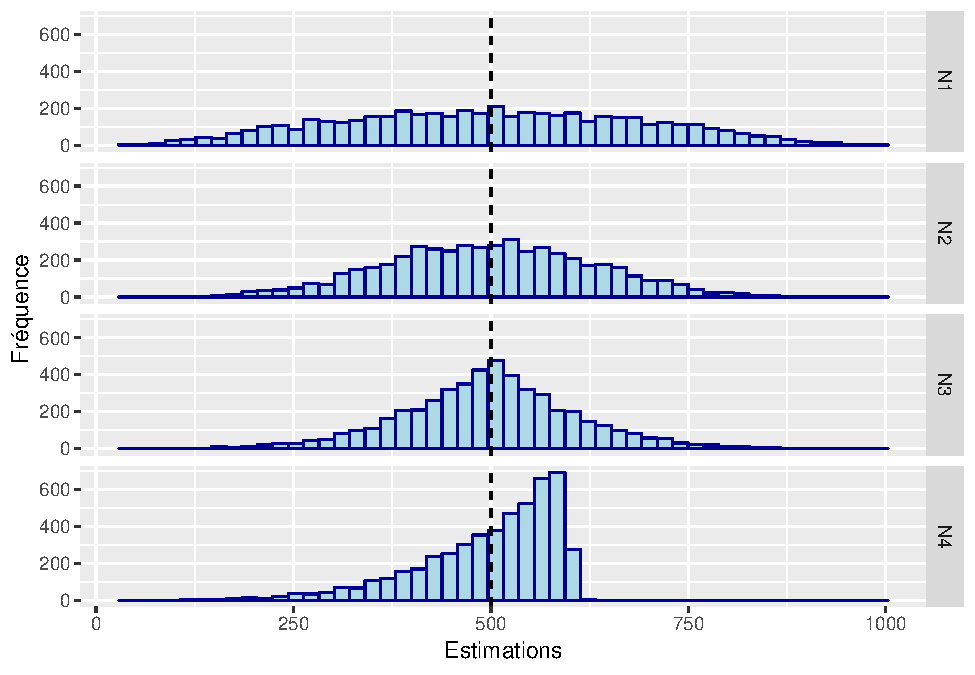
\includegraphics[width=0.9\linewidth]{serial_number_amq_files/figure-latex/ech-taille-5-1} \caption{Représentation sous forme d'histogrammes de 5 000 échantillons de taille 5, pour les quatres estimateurs}\label{fig:ech-taille-5}
\end{figure}

\appendix

\hypertarget{rappels}{%
\section{\texorpdfstring{Rappels
\label{rappel_esperance}}{Rappels }}\label{rappels}}

Voici quelques propriétés élémentaires concernant l'espérance, la
variance et la covariance de variables aléatoires.

\begin{itemize}
\item
  L'espérance d'une variable aléatoire constante est égale à cette
  constante; par exemple, si \(k\) est une constante, alors
  \(\mathbb{E}(k)=k\).
\item
  L'espérance est un opérateur linéaire. Pour deux variables aléatoires
  quelconques \(X\) et \(Y\) (définies sur le même espace probabiliste)
  et pour deux nombres réels \(a\) et \(b\) alors
  \(\mathbb{E}(aX+bY)=a\mathbb{E}(X)+b\mathbb{E}(Y)\).
\item
  La variance d'une variable aléatoire peut être calculée de la façon
  suivante \(Var(X)=\mathbb{E}(X^2)-\lr{\mathbb{E}(X)}^2\).
\item
  La variance
\end{itemize}

TODO

\hypertarget{calcul-de-probabilites}{%
\section{\texorpdfstring{Calcul de probabilités
\label{calculs_proba}}{Calcul de probabilités }}\label{calcul-de-probabilites}}

TODO

Nous voulons calculer la probabilité reliée à l'événement \(X_{(A)}=i\),
c'est-à-dire l'événement où l'unité statistique \(X_{(A)}=i\). Pour bien
comprendre la situation, nous allons utiliser le schéma ci-dessous:
\begin{align*}
\underbrace{X_{(1)} <  X_{(2)} < \ldots < X_{(A-1)}}_{A-1 \text{ éléments}} 
< X_{(A)} 
< \underbrace{X_{(A+1)} < \ldots < X_{(n-1)} < X_{(n)}}_{n-A \text{ éléments}}
\end{align*} Nous remarquons que \(A\in\set{1,2,3,\ldots, n}\) et
\(i\in\set{A,A+1,A+2,\ldots,N-n+A}\). En effet, la valeur de \(i\) ne
peut pas être plus petite que \(A\) car il y a toujours \(A-1\) valeurs
plus petites que \(A\). De plus, \(A\) ne peut pas être plus grande que
\(N-n+A\) car il y a toujours \(N-n+A-1\) valeurs plus grandes que
\(A\).

Pour calculer les probabilités, il faut se rappeler que nous devons
choisir \(A-1\) éléments parmi \(i-1\), ce qui correspond à
\(\binom{i-1}{A-1}\). De plus, nous devons choisir \(n-A\) éléments
parmi \(N-i\), ce qui correspond à \(\binom{N-i}{n-A}\). Enfin, nous
choisissons un échantillon de taille \(n\) parmi une population de
taille \(N\), ce qui correspond à \(\binom{N}{n}\). Nous avons donc:
\begin{align*}
P(X_{(A)}=i) &= \dfrac{\binom{i-1}{A-1}\binom{N-i}{n-A}}{\binom{N}{n}} \qquad \text{où } i=A,A+1,\ldots,N-n+A
\end{align*} Puisque les probabilités précédentes doivent sommer à un,
nous avons: \begin{align}
\sum_{i=A}^{N-n+A} P(X_{(A)}=i) &= 1 \nonumber\\
\sum_{i=A}^{N-n+A} \dfrac{\binom{i-1}{A-1}\binom{N-i}{n-A}}{\binom{N}{n}} &= 1 \nonumber\\
\sum_{i=A}^{N-n+A} \binom{i-1}{A-1}\binom{N-i}{n-A} &= \binom{N}{n} \label{eq:sumxA}
\end{align}

Nous pouvons maintenant calculer l'espérance de \(X_{(A)}\). Nous avons:
\begin{align}
E(X_{(A)}) &= \sum_{i=A}^{N-n+A} iP(X_{(A)}=i) \nonumber\\
&= \sum_{i=A}^{N-n+A} i\dfrac{\binom{i-1}{A-1}\binom{N-i}{n-A}}{\binom{N}{n}} \nonumber\\
&= \dfrac{1}{\binom{N}{n}}\sum_{i=A}^{N-n+A} i\binom{i-1}{A-1}\binom{N-i}{n-A} \nonumber\\
&= \dfrac{1}{\binom{N}{n}}\sum_{i=A}^{N-n+A} A\binom{i}{A}\binom{N-i}{n-A} 
\comeq{car $\binom{n}{k}=\dfrac{n}{k}\binom{n-1}{k-1}$} \nonumber\\
&= \dfrac{A}{\binom{N}{n}}\sum_{i=A}^{N-n+A} \binom{i}{A}\binom{N-i}{n-A} \nonumber\\
&= \dfrac{A}{\binom{N}{n}}\binom{N+1}{n+1} \comeq{par l'équation \ref{eq:sumxA} et changement d'indice} \nonumber\\
&= \dfrac{A(N+1)}{n+1} \label{eq:esperancexA}
\end{align}

\bigskip

\bibliographystyle{alpha}
\begin{thebibliography}{10}

\bibitem{Johnson} Roger W. Johnson (1994). Estimating the Size of a Population, {\em Teaching Statistics, 16}, (no. 2), pages 50-52.

\bibitem{Goodman1952} Leo A. Goodman (1952). Serial Number Analysis, {\em Journal of the American Statistical Association, 47}, (no. 260), pages 622-634.

\bibitem{Goodman1954} Leo A. Goodman (1954). Some Practical Techniques in Serial Number Analysis, {\em Journal of the American Statistical Association, 49}, (no. 265), pages 97-112.

\bibitem{Roberts1967} Harry V. Roberts (1967). Informative Stopping Rules and Inferences about Population Size, {\em Journal of the American Statistical Association, 62}, (no. 319), pages 763-775.

\bibitem{Volz2008} Arthur G. Volz (2008). A Soviet Estimate of German Tank Production, {\em The Journal of Slavic Military Studies, 21}, (no. 3), pages 588-590.

\bibitem{Ruggles1947} Richard Ruggles and Henry Brodie (1947). An Empirical Approach to Economic Intelligence in World War II, {\em Journal of the American Statistical Association, 42}, (no. 237), pages 72-91.

\bibitem{Hohle2006} Michael Höhle and Leonhard Held (2006). Bayesian estimation of the size of a population, {\em Technical report, SFB 386}, (no. 399).

\bibitem{commodore64} Pagetable.com (4 février 2011). {\em How many Commodore 64 were really sold?}. Récupéré le 17 octobre 2018:  \href{https://web.archive.org/web/20160306232450/http://www.pagetable.com/?p=547}{https://web.archive.org/web/20160306232450/http://www.pagetable.com/?p=547}

\bibitem{iphone} Charles Artur (8 octobre 2008). {\em Why iPhones are just like German tanks.}. Récupéré le 17 octobre 2018: \href{https://www.theguardian.com/technology/blog/2008/oct/08/iphone.apple}{https://www.theguardian.com/technology/blog/2008/oct/08/iphone.apple}

\bibitem{Hinno} Risto Hinno (14 février 2015). {\em German tank problem.}. Récupéré le 19 octobre 2018:  \href{http://bit.ly/2P7U9dE}{http://bit.ly/2P7U9dE}

\bibitem{WikiGermanTank} {\em German tank problem.}. Récupéré le 19 octobre 2018:  \href{https://en.wikipedia.org/wiki/German_tank_problem}{https://en.wikipedia.org/wiki/GermanTankProblem}

\end{thebibliography}


\end{document}
